\documentclass[a4paper,12pt]{article}

\usepackage{mystyle}

\graphicspath{ {images/} }


% https://tex.stackexchange.com/questions/5461/is-it-possible-to-change-the-size-of-an-arrowhead-in-tikz-pgf
\usetikzlibrary{arrows.meta}

% https://tex.stackexchange.com/questions/261591/arrow-above-text-like-widehat
\usepackage{esvect}

% https://tex.stackexchange.com/questions/32501/how-to-get-a-good-divisible-by-symbol
\DeclareRobustCommand{\divby}{%
  \mathrel{\vbox{\baselineskip.65ex\lineskiplimit0pt\hbox{.}\hbox{.}\hbox{.}}}%
}


\definecolor{my-green}{RGB}{0, 153, 0}


\author{Алексеев Василий}
\title{Семинар 2}
\date{8 сентября 2021}


\begin{document}
  \maketitle
  
  \tableofcontents

  \thispagestyle{empty}
  
  \newpage
  
  \pagenumbering{arabic}


  \section{Вектора (-ы?)}
  
  Вектор~---~направленный отрезок (\ref{fig:vector}).
  Вектор можно обозначать одной строчной буквой, например $\bds a$, или двумя: началом и концом, например $\vv{AB}$.
  
  \begin{figure}[h]
    \centering
    
    \begin{tikzpicture}
      \draw[-{Latex[length=5mm, width=2mm]}, thick] (0,0) node[anchor=north west]{$A$} -- (5,5) node[anchor=north west]{$B$};
      \draw[ultra thick, fill] (0,0) circle[radius=0.05];
    \end{tikzpicture}
    
    \caption{Вектор характеризуется направлением и величиной.}
    \label{fig:vector}
  \end{figure}
  
  \begin{definition}[Коллинеарность]
    Два ненулевых вектора $\bds a$ и $\bds b$ называются \emph{коллинеарными}, если существует прямая, которой они параллельны (\ref{fig:collinearity}).
    Коллинеарность обозначается $\bds a \hm\parallel \bds b$.
    Если при этом $\bds a$ и $\bds b$ направлены в одну сторону, то можно писать $\bds a \hm\upuparrows \bds b$,
    если в разные стороны~---~$\bds a \hm\updownarrows \bds b$.
    Нулевой вектор коллинеарен любому вектору.
  \end{definition}
  
  \begin{figure}[h]
    \centering
    
    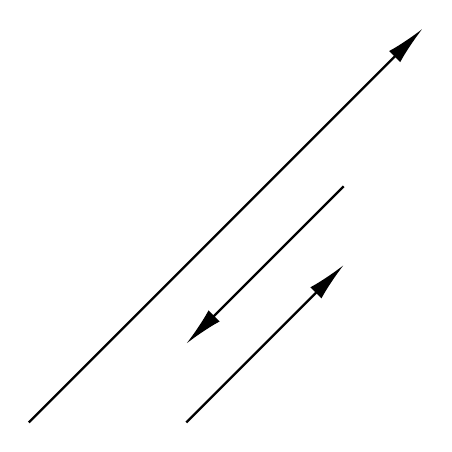
\begin{tikzpicture}
      \draw[-{Latex[length=5mm, width=2mm]}, thick] (0,0) -- (5,5);
      \draw[{Latex[length=5mm, width=2mm]}-, thick] (2,1) -- (4,3);
      \draw[-{Latex[length=5mm, width=2mm]}, thick] (2,0) -- (4,2);
    \end{tikzpicture}
    
    \caption{Коллинеарные вектора.}
    \label{fig:collinearity}
  \end{figure}
  
  \begin{definition}[Компланарность]
    Три ненулевых вектора $\bds a$, $\bds b$ и $\bds c$ называются \emph{компланарными}, если существует плоскость, которой они параллельны (\ref{fig:coplanarity}).
    Три вектора, два из которых ненулевые, а третий нулевой, всегда компланарны.
  \end{definition}
  
  \begin{figure}[h]
    \centering
    
    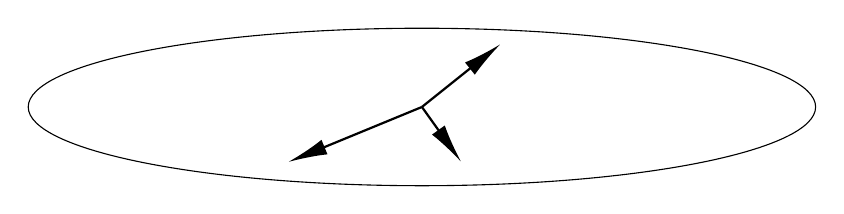
\begin{tikzpicture}
      \draw (0,0) ellipse (5cm and 1cm);
      \draw[-{Latex[length=5mm, width=2mm]}, thick] (0,0) -- (1,0.8);
      \draw[-{Latex[length=5mm, width=2mm]}, thick] (0,0) -- (0.5,-0.7);
      \draw[-{Latex[length=5mm, width=2mm]}, thick] (0,0) -- (-1.7,-0.7);
    \end{tikzpicture}
    
    \caption{Компланарные вектора.}
    \label{fig:coplanarity}
  \end{figure}
  
  \begin{definition}[Равенство векторов]
    Будем считать два вектора $\bds a$ и $\bds b$ равными, если они
    \begin{itemize}
      \item равны по длине $|\bds a| = |\bds b|$
      \item одинаково направлены $\bds a \upuparrows \bds b$
    \end{itemize}
    Точка приложения при равенстве не учитывается\footnote{То есть получается, что можно нарисовать несколько несовпадающих, но равных векторов. Хотя в зависимости от конкретной задачи может быть важным различать векторы с разной точкой приложения. Например, в физике, при действии сил на тело.}.
  \end{definition}
  
  На множестве векторов можно определить следующие операции:
  \begin{itemize}
    \item Сложение векторов (по правилу треугольника):  % TODO: pic
      \[
        \vv{AB} + \vv{BC} = \vv{AC}
      \]
    \item Умножение вектора $\bds a$ на число $\alpha \in \RR$.
      Результирующий вектор обозначается как $\alpha \bds a$ и определяется свойствами:
      \[
        \left\{
          \begin{aligned}
            &|\alpha \bds a| = |\alpha| \cdot |\bds a|\\
            &\left\{
               \begin{aligned}
                 &\alpha \bds a \upuparrows \bds a, \alpha > 0\\
                 &\alpha \bds a \updownarrows \bds a, \alpha < 0
               \end{aligned}
             \right.
          \end{aligned}
        \right.
      \]
      (то есть при $\alpha \hm= 0$ будет нулевой вектор, и которого нет определённого направления).
  \end{itemize}
  
  Множество векторов в $\RR^3$ с введёнными операциями сложения и умножения на число из $\RR$ образуют линейное пространство\footnote{Формально $\RR^3$~---~это не векторы как направленные отрезки, а столбцы из чисел. Но мы будем использовать обозначения $\RR^2$ и $\RR^3$ не только для векторов-столбцов, но и для векторов~---~направленных отрезков на плоскости и в трёхмерном пространстве соответственно.}.
  
  \begin{remark}
    В чём можно убедиться, проверив следующие свойства операций, введённых на множестве векторов (обозначим за $V$ векторы трёхмерного пространства):
    \begin{enumerate}
      \item $\bds a + (\bds b + \bds c) = (\bds a + \bds b) + \bds c$, $\forall \bds a, \bds b, \bds c \in V$ (ассоциативность сложения).
      \item $\bds a + \bds b = \bds b + \bds a$, $\forall \bds a, \bds b \in V$ (коммутативность сложения).
      \item $\exists \bds 0 \in V: \bds 0 + \bds a = \bds a$, $\forall \bds a \hm\in V$.
      \item $\forall \bds a \in V\, \exists {-\bds a} \in V: \bds a + ({-\bds a}) = \bds 0$.
      \item $\alpha (\beta \bds a) = (\alpha \beta) \bds a$, $\forall \alpha, \beta \in \RR$, $\forall \bds a \hm\in V$ (ассоциативность умножения на скаляр).
      \item $1 \cdot \bds a = \bds a$, $\forall \bds a \in V$.
      \item $(\alpha + \beta) \bds a = \alpha \bds a + \beta \bds a$, $\forall \alpha, \beta \hm\in \RR$, $\bds a \hm\in V$ (дистрибутивность умножения матрицы на число относительно сложения чисел).
      \item $\alpha (\bds a + \bds b) = \alpha \bds a + \alpha \bds b$, $\forall \alpha \hm\in \RR$, $\bds a, \bds b \hm\in V$ (дистрибутивность умножения матрицы на число относительно сложения матриц).
    \end{enumerate}
  \end{remark}
  
  Но рассмотрим векторы на одной прямой: сложение и умножение на число не выводят с прямой.
  То же самое с векторами на плоскости: сложение и умножение на число даёт вектор, также лежащий в той же плоскости.
  Таким образом, не только векторы из всего $\RR^3$ образуют линейное пространство, но и векторы, параллельные одной прямой, и векторы, параллельные одной плоскости.
  Множество векторов из одного нулевого вектора также образуют линейное пространство.
  Таким образом,
  \begin{itemize}
    \item нульмерное векторное пространство~---~нулевой вектор
    \item одномерное векторное пространство
      \[
        \{\bds v \in \RR^3 \mid \bds v \parallel l\}, \quad \mbox{$l$~---~прямая}
      \]
    \item двумерное векторное пространство
      \[
        \{\bds v \in \RR^3 \mid \bds v \parallel \alpha\}, \quad \mbox{$\alpha$~---~плоскость}
      \]
    \item трёхмерное векторное пространство~---~$\RR^3$
  \end{itemize}
  
  \begin{definition}
    Линейная комбинация векторов $\bds a_1, \ldots, \bds a_n$:
    \[
      \alpha_1 \bds a_1 + \ldots + \alpha_n \bds a_n, \quad \alpha_i \in \RR, 1 \leq i \leq n
    \]
    
    Нетривиальная линейная комбинация~---~когда хотя бы один их коэффициентов $\alpha_i$ отличен от нуля:
    $\sum\limits_{i=1}^n \alpha_i^2 \hm> 0$.
  \end{definition}
  
  \begin{definition}[Линейно зависимая система векторов]
    Система векторов $\bds a_1, \ldots, \bds a_n$ называется линейно зависимой, если существует их нетривиальная линейная комбинация, равная нулевому вектору:
    \[
      \left\{
        \begin{aligned}
          &\alpha_1 \bds a_1 + \ldots + \alpha_n \bds a_n = \bds 0\\
          &\alpha_1^2 + \ldots + \alpha_n^2 > 0
        \end{aligned}
      \right.
    \]
  \end{definition}
  
  \begin{example}
    Система из одного нулевого вектора линейно зависима.
  \end{example}
  
  \begin{theorem}
    Система из $k > 1$ вектора линейно зависима тогда и только тогда, когда один из векторов системы представим как линейная комбинация остальных.
  \end{theorem}
  
  \begin{proof}
    Пусть $\bds a_1, \ldots, \bds a_n$~---~линейно зависимы.
    Это значит, что
    \[
      \alpha_1 \bds a_1 + \ldots + \alpha_n \bds a_n = \bds 0
    \]
    и некоторый $\alpha_j \hm{\not=} 0$.
    Поэтому
    \[
      \alpha_j = \sum\limits_{\substack{1 \leq i \leq n\\i \not= j}} -\frac{\alpha_i}{\alpha_j} \bds a_i
    \]
    
    И наоборот, пусть некоторый $\bds a_j$ представим как линейная комбинация остальных векторов из набора с коэффициентами $\alpha_i'$:
    \[
      \bds a_j = \sum\limits_{\substack{1 \leq i \leq n\\i \not= j}} \alpha_i' \bds a_i
    \]
    Тогда
    \[
      \alpha_1' \bds a_1 + \ldots + (-1) \cdot \bds a_j + \ldots + \alpha_n' \bds a_n = \bds 0
    \]
    и по крайней мере один коэффициент $-1$ при разложении нуля $\bds 0$ в линейную комбинацию векторов $\{\bds a_i\}_{i=1}^n$ не равен нулю.
  \end{proof}
  
  \begin{theorem}\label{theo:linear-dependence-criteria}
    Критерии линейной зависимости систем векторов:
    \begin{itemize}
      \item Один вектор линейно зависим $\Leftrightarrow$ это нулевой вектор.
      \item Два вектора линейно зависимы $\Leftrightarrow$ эти векторы коллинеарны.
      \item Три вектора линейно зависимы $\Leftrightarrow$ эти векторы компланарны.
      \item Любые четыре вектора линейно зависимы.
    \end{itemize}
  \end{theorem}
  
  \begin{definition}[Базис]
    Базисом в пространстве называется
    \begin{itemize}
      \item упорядоченная (векторы перенумерованы)
      \item линейно независимая (только тривиальная линейная комбинация векторов равна нулевому вектору)
      \item полная (любой вектор пространства можно представить как их линейную комбинацию)
    \end{itemize}
    система векторов.
  \end{definition}
  
  Из теоремы (\ref{theo:linear-dependence-criteria}) следует, что
  \begin{itemize}
    \item В нулевом пространстве не существует базиса.
    \item В одномерном пространстве ненулевой вектор образует базис.
    \item В двумерном пространстве пара неколлинеарных векторов образует базис.
    \item В трёхмерном пространстве тройка некомпланарных векторов образует базис.
  \end{itemize}
  
  \begin{remark}
    При заданном базисе $\{\bds e_1, \ldots, \bds e_n\}$ каждому вектору можно поставить в соответствие набор чисел~---~коэффициентов при разложении вектора по базису $\bds a \hm= \alpha_1 \bds e_1 \hm+ \ldots \hm+ \alpha_n \bds e_n$:
    \[
        \bds a \leftrightarrow (\alpha_1, \ldots, \alpha_n) \in \RR^n
    \]
    Соответствие взаимно однозначное (каждому вектору соответствует один координатный столбец и каждому столбцу соответствует один вектор), потому что базисная система векторов линейно независима.
    Более того, сложение векторов~---~направленных отрезков соответствует сложению их координатных столбцов (у вектора~---~результата сложения координатный столбец в базисе равен сумме координатных столбцов векторов-слагаемых).
    И умножение вектора на число соответствует умножению его координатного столбца на это же самое число.
    То есть между векторами~---~направленными отрезками и векторами~---~координатными столбцами соответствие не просто взаимно однозначное, но такое, при котором ещё сохраняются линейные операции.
  \end{remark}
  
  \begin{definition}[Система координат]
    Декартовой системой координат\footnote{Помимо декартовой, есть и другие системы координат. Например полярная, когда положение точки на плоскости определяется по расстоянию $r$ от начала координат $O$ и по углу $\phi$, которое направление из начала координат на точку образует с выбранным направлением $\bds l$: $\bds a \hm\leftrightarrow (r, \phi)$.} называется совокупность точки и базиса $O; \bds e_1, \ldots, \bds e_n$.
    Точка $O$ называется началом отчёта.
  \end{definition}
  
  \begin{remark}
    При заданной системе координат $O; \bds e_1, \ldots, \bds e_n$ каждой точке $A$ можно поставить в соответствие набор чисел~---~компонент радиуса-вектора точки в базисе $\vv{OA} \hm= \alpha_1 \bds a_1 \hm+ \ldots \hm+ \alpha_n \bds a_n$:
    \[
      A \leftrightarrow (\alpha_1, \ldots, \alpha_n) \in \RR^n
    \]
  \end{remark}
  
  
  \subsection{Задачи}
  
  \begin{problem}[1.6]
    $\bds a(-5, -1), \bds b(-1, 3)$~---~проверить, что система из двух векторов образует базис.
    Разложить $\bds c(-1, 2)$ и $\bds d(2, -6)$ по этому базису.
  \end{problem}
  
  \begin{solution}
    Все векторы заданы компонентами в некотором неизвестном базисе $(\bds e_1, \bds e_2)$.
    
    Для доказательства того, что $\bds a$ и $\bds b$ вместе образуют базис, достаточно проверить их линейную независимость.
    Для проверки же линейной независимости векторов, можно проверить линейную независимость соответствующих им столбцов.
    Иными словами, надо проверить, что координатные столбцы $\bds a$ и $\bds b$ в базисе $(\bds e_1, \bds e_2)$ неколлинеарны:
    \[
      (-5, -1) = \alpha (-1, 3) \Rightarrow \alpha \in \noth
    \]
    
    Теперь разложим, например, вектор $\bds c$ по $\bds a$ и $\bds b$ (с вектором $\bds d$ будет аналогично):
    \[
      \bds c = \alpha \bds a + \beta \bds b
    \]
    \[
      \begin{pmatrix}
        -1 \\ 2
      \end{pmatrix}
      = \alpha \begin{pmatrix}
          -5 \\ -1
        \end{pmatrix}
        + \beta \begin{pmatrix}
          -1 \\ 3
        \end{pmatrix}
      = \begin{pmatrix}
          -5\alpha - \beta\\
          -\alpha + 3\beta
        \end{pmatrix}
      = \begin{pmatrix}
          -5 -1\\
          -1 + 3
        \end{pmatrix}
        \begin{pmatrix}
          \alpha \\ \beta
        \end{pmatrix}
    \]
    
    Решаем получившуюся систему методом Крамера:
    \[
      \Delta = \begin{vmatrix}
        -5 & -1\\
        -1 & 3
      \end{vmatrix} = -16
    \]
    \[
      \Delta_1 = \begin{vmatrix}
        -1 & -1\\
        -2 & 3
      \end{vmatrix} = -1
    \]
    \[
      \Delta_2 = \begin{vmatrix}
        -5 & -1\\
        -1 & 2
      \end{vmatrix} = -11
    \]
    
    И коэффициенты разложения:
    \[
      \left\{
        \begin{aligned}
          &\alpha = \frac{\Delta_1}{\Delta} = \frac{1}{16}\\
          &\beta = \frac{\Delta_2}{\Delta} = \frac{11}{16}
        \end{aligned}
      \right.
    \]
  \end{solution}
  

  \begin{problem}[1.11(1)]
    Компланарны ли $\bds l, \bds m, \bds n$?
    \begin{equation}
      \label{eq:problem1.11}
      \left\{
        \begin{aligned}
          &\bds l = \bds a + \bds b + \bds c\\
          &\bds m =          \bds b + \bds c\\
          &\bds n = -\bds a         + \bds c
        \end{aligned}
      \right.
    \end{equation}
    (про векторы $\bds a, \bds b, \bds c$ при этом известно, что они некомпланарны).
  \end{problem}
  
  \begin{solution}
    \vphantom{}\par
    
    \emph{Способ 1.}
    
    \medskip
    
    Векторы $\bds a, \bds b, \bds c$ некомпланарны $\Rightarrow$ они линейно независимы, и в трёхмерном пространстве образуют базис.
    Компланарность $\bds l, \bds m, \bds n$ равносильна их линейной зависимости:
    \[
      \alpha \bds l + \beta \bds m + \gamma \bds n = \bds 0
    \]
    
    Что, в свою очередь, равносильно линейной зависимости (с теми же коэффициентами) их координатных столбцов в базисе:
    \[
      \alpha \begin{pmatrix}
        1 \\ 1 \\ 1
      \end{pmatrix}
      + \beta \begin{pmatrix}
        0 \\ 1 \\ 1
      \end{pmatrix}
      + \gamma \begin{pmatrix}
        -1 \\ 0 \\ 1
      \end{pmatrix}
      = 0
    \]
    
    Или, в более компактном виде:
    \[
      \begin{pmatrix}
        1 & 0 & -1\\
        1 & 1 & 0\\
        1 & 1 & 1
      \end{pmatrix}
      \begin{pmatrix}
        \alpha \\ \beta \\ \gamma
      \end{pmatrix}
      = 0
    \]
    
    Очевидно, определитель матрицы системы не равен нулю ($\Delta \hm= 1$).
    То есть, по Крамеру, решение системы существует и единственно.
    Но нулевой вектор $(\alpha, \beta, \gamma)^T \hm= (0, 0, 0)^T$ точно является решением (система однородная).
    Поэтому единственное решение:
    \[
      (\alpha, \beta, \gamma)^T \hm= (0, 0, 0)^T
    \]
    Но это значит, что система векторов $\bds l$, $\bds m$, $\bds n$ линейно независима (только их тривиальная линейная комбинация, где все коэффициенты нулевые, может быть равна нулевому вектору).
    То есть векторы некомпланарны.
    
    \bigskip
    
    \emph{Способ 2.}
    
    \medskip
    
    (Как было замечено на семинаре) можно было просто попробовать решить систему (\ref{eq:problem1.11}).
    В системе этой участвуют не числа (как обычно), а векторы (направленные отрезки).
    Но так как линейные операции (сложение и умножение на число) работают одинаково, что с векторами, что с числами, то мы можем попробовать решить систему относительно векторов $\bds a$, $\bds b$, $\bds c$.
    Что нам это даст, если получится выразить $\bds a$, $\bds b$, $\bds c$ через $\bds l$, $\bds m$, $\bds n$ (или если не получится)?
    Система $\bds a$, $\bds b$, $\bds c$ образует базис.
    То есть они линейно независимы и любой вектор пространства можно представить как их линейную комбинацию.
    Если $\bds a$, $\bds b$, $\bds c$ выражаются через $\bds l$, $\bds m$, $\bds n$, то потому и любой вектор пространства тоже разложится по $\bds l$, $\bds m$, $\bds n$.
    То есть система векторов $\bds l$, $\bds m$, $\bds n$ тоже полная.
    
    (...Внимательно смотрим на систему из условия задачи, понимаем, что она решается относительно $\bds a$, $\bds b$, и $\bds c$...)
    
    Могут ли теперь $\bds l$, $\bds m$, $\bds n$ быть линейно зависимыми?
    Допустим, да.
    Тогда максимальное количество линейно независимых векторов среди $\bds l$, $\bds m$, $\bds n$~---~это два вектора или вообще один.
    В любом случае, если $\bds l$, $\bds m$, $\bds n$ линейно зависимы, то они компланарны (\ref{theo:linear-dependence-criteria}).
    Но тогда в трёхмерном пространстве можно будет найти вектор, который по $\bds l$, $\bds m$, $\bds n$ разложен быть не может (который не лежит в плоскости $\bds l$, $\bds m$, $\bds n$).
    Получаем противоречие с уже доказанной полнотой.
    
    То есть $\bds l$, $\bds m$, $\bds n$, линейно независимы, а потому некомпланарны.
  \end{solution}
  
  
  \begin{problem}[1.21]
    В $\triangle ABC$ точка $M$~---~середина стороны $AC$.
    Также известно, что $K \hm\in [AB]$ и $AK \hm: KB \hm= 3 \hm: 5$.
    И ещё $L \hm\in [BC]$ и $BL \hm: LC \hm= 2 \hm: 3$.
    Векторы $\vv{OA}, \vv{OB}$~---~базис.
    
    Надо найти координаты вектора $\vv{BM}$ в базисе $\{\vv{AL}, \vv{CK}\}$.
  \end{problem}
  
  \begin{solution}
    Очевидно, векторы $\{\vv{AL}, \vv{CK}\}$, которые предлагается взять в качестве базисных, неколлинеарны, а потому в самом деле образуют базис на плоскости (\ref{fig:triangle-for-problem-1-21}).
    
    \begin{figure}[h]
      \centering
      
      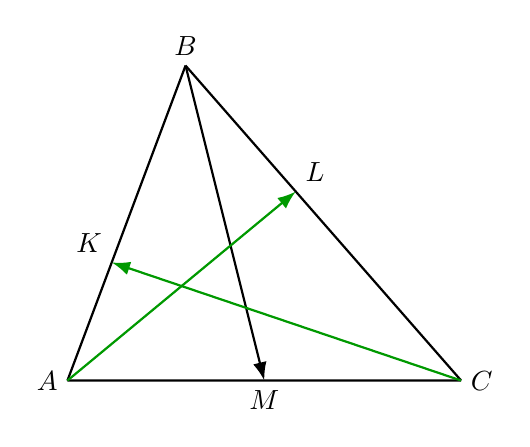
\begin{tikzpicture}
        \node[anchor=east] at (0,0) {$A$};
        \coordinate (A) at (0,0);
        
        \node[anchor=west] at (5,0) {$C$};
        \coordinate (C) at (5,0);
        
        \node[anchor=south] at (1.5,4) {$B$};
        \coordinate (B) at (1.5,4);
        
        \draw[-,thick] (A) -- (C)
                       (C) -- (B)
                       (B) -- (A);
        
        \node[anchor=north] at (2.5,0) {$M$};
        \coordinate (M) at (2.5,0);
        
        \node[anchor=south west] at (2.9,2.4) {$L$};
        \coordinate (L) at (2.9,2.4);
        
        \node[anchor=south east] at (0.5625,1.5) {$K$};
        \coordinate (K) at (0.5625,1.5);
        
        \draw[-Latex,thick]          (B) -- (M);
        \draw[-Latex,thick,my-green] (A) -- (L);
        \draw[-Latex,thick,my-green] (C) -- (K);
      \end{tikzpicture}
      
      \caption{Треугольник $\triangle ABC$ и точки $M$, $K$ и $L$, делящие его стороны в заданном отношении.}
      \label{fig:triangle-for-problem-1-21}
    \end{figure}
    
    Задачу можно бы было решить, отложив векторы $\vv{BM}$ и $\{\vv{AL}, \vv{CK}\}$ от одной точки и далее воспользовавшись правилом треугольника сложения векторов (\ref{fig:physi-way}).
    Но точное решение, очевидно, надо получить, воспользовавшись соотношениями между отрезками, на которые точки делят стороны треугольника...
    
    Какие соотношения можно выписать для векторов?
    Можно представить $\vv{BM}$ как сумму чего-то:
    \[
      \left\{
        \begin{aligned}
          &\vv{BM} = \vv{BA} + \vv{AM}\\
          &\vv{BM} = \vv{BC} + \vv{CM}
        \end{aligned}
      \right.
    \]
    
    Потом можно ещё выписать несколько соотношений с известными $\vv{CK}$ и $\vv{AL}$:
    \[
      \left\{
        \begin{aligned}
          &\vv{CK} = \vv{CA} + \vv{AK}\\
          &\vv{AL} = \vv{AC} + \vv{CL}
        \end{aligned}
      \right.
    \]
    
    Очевидно, из соотношений с $\vv{BM}$ можно выразить $\vv{AK}$ и $\vv{CL}$ через $\vv{BM}$.
    И потом подставить это в систему с $\vv{CK}$ и $\vv{AL}$.
    Получится система из двух уравнений с двумя неизвестными ($\vv{BM}$ и, например, $\vv{AC}$).
    Которую уже можно решить...
    
    \begin{figure}[h]
      \centering
      
      \begin{tikzpicture}
        \coordinate (A) at (0,0);
        \coordinate (C) at (0,0);
        
        \node[anchor=south] at (0,0) {$B$};
        \coordinate (B) at (0,0);
   
        \node[anchor=west] at (1,-4) {$M$};
        \coordinate (M) at (1,-4);
        
        \node[anchor=south] at (2.9,2.4) {$\bds e_1$};
        \coordinate (L) at (2.9,2.4);
        
        \node[anchor=south] at (-4.4375,1.5) {$\bds e_2$};
        \coordinate (K) at (-4.4375,1.5);
  
        \draw[-Latex,thick]          (B) -- (M);
        \draw[-Latex,thick,my-green] (A) -- (L);
        \draw[-Latex,thick,my-green] (C) -- (K);
        
        \draw[thick,dotted]          (B) -- (-5.8,-4.8);
        \draw[thick,dotted]          (L) -- (4.35,3.6);
        \draw[thick,dotted]          (M) -- (-5.65625,-1.75);
        
        \coordinate (X) at (-3.142,-2.6);
        \node[above=0.5em of X] at (X) {$\alpha \bds e_1$};  % TODO: fix spacing here (read https://tex.stackexchange.com/questions/43807/what-are-the-ways-one-can-control-spacing-between-nodes-in-tikz ?)
        \node[anchor=north east] at (M) {$\beta \bds e_2$};
        
        \draw[-Latex,thick,dotted,my-green]   (B) -- (X);
        \draw[-Latex,thick,dotted,my-green]   (X) -- (M);
      \end{tikzpicture}
      
      \caption{Разложить вектор по базису можно с помощью правила треугольника сложения векторов.}
      \label{fig:physi-way}
    \end{figure}
    
    А вообще, стоит про себя на всякий случай понимать, что треугольник однозначно определяется длинами дрёх его сторон (либо двумя сторонами и углом между ними).
    Обладая этими тремя значениями, дальше в треугольнике можно посчитать что угодно.
    
    Два вектора, связанные с треугольником, по условию даны.
    Ещё точно известно соотношение между векторами, отложенными на сторонах треугольника ($\vv{AB} \hm+ \vv{BC} \hm+ \vv{CA} \hm= \bds 0$).
    Получается, есть три неизвестных (векторы~---~стороны треугольника) и три соотношения между ними.
    Откуда точно можно всё найти.
  \end{solution}
  
  
  \section{Дополнение}
  
  \subsection{Про матричное умножение}
  
  Почему матричное умножение введено именно так: $C_{m\times n} \hm= A_{m\times p}B_{p\times n}$, $c_{ij} \hm= \sum\limits_{k=1}^p a_{ik} b_{kn},\ 1 \hm\leq i \hm\leq m, 1 \hm\leq j \hm\leq n$?
  
  Пусть есть ортонормированный\footnote{Вектора взаимно перпендикулярны и по длине равны единице $1$.} базис $\bds e_1, \bds e_2$.
  Повернём вектор $\bds v$ с компонентами $(1, 0)$ на угол $45$ градусов против часовой стрелки (\ref{fig:turning-vector}).
  
  \begin{figure}[h]
    \centering
    
    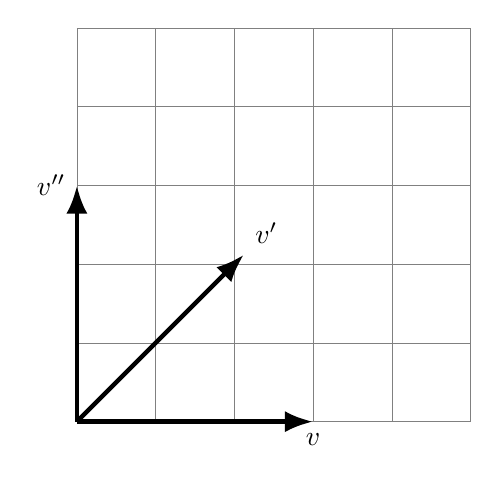
\begin{tikzpicture}
      \draw[step=1cm,gray,very thin] (0,0) grid (5,5);
      \draw[-Latex,ultra thick] (0,0) -- (3,0) node[anchor=north]{$\boldsymbol{v}$};
      \draw[-Latex,ultra thick] (0,0) -- (2.121,2.121) node[anchor=south west]{$\boldsymbol{v'}$};
      \draw[-Latex,ultra thick] (0,0) -- (0,3) node[anchor=east]{$\boldsymbol{v''}$};
    \end{tikzpicture}
    
    \caption{Несколько поворотов вектора $\bds v$ на $45$ градусов против часовой стрелки.}
    \label{fig:turning-vector}
  \end{figure}
  
  Получим вектор $\left(1/\sqrt{2}, 1/\sqrt{2}\right)$.
  Проверим, что матрица $\left(\begin{smallmatrix}1/\sqrt{2} & -1/\sqrt{2}\\ 1/\sqrt{2} & 1/\sqrt{2}\end{smallmatrix}\right)$ как раз задаёт нужное преобразование:
  \[
    v'
    = A \bds v
    = \begin{pmatrix}
        1/\sqrt{2} & -1/\sqrt{2}\\
        1/\sqrt{2} & 1/\sqrt{2}
      \end{pmatrix}
      \begin{pmatrix}
        1 \\ 0
      \end{pmatrix}
    = \begin{pmatrix}
        1/\sqrt{2} \\ 1/\sqrt{2}
      \end{pmatrix}
  \]
  
  Снова повернём вектор на угол $45$ градусов против часовой стрелки.
  Должны получить вектор с компонентами $\left(\begin{smallmatrix}0 \\ 1\end{smallmatrix}\right)$:
  \[
    v''
    = A \bds v'
    = \begin{pmatrix}
        1/\sqrt{2} & -1/\sqrt{2}\\
        1/\sqrt{2} & 1/\sqrt{2}
      \end{pmatrix}
      \begin{pmatrix}
        1/\sqrt{2} \\ 1/\sqrt{2}
      \end{pmatrix}
    = \begin{pmatrix}
        0 \\ 1
      \end{pmatrix}
  \]
  
  Какой матрицей задаётся поворот сразу на $90$ градусов против часовой стрелки?
  Как из вектора
  $\left(\begin{smallmatrix}1 \\ 0\end{smallmatrix}\right)$
  сразу получить вектор
  $\left(\begin{smallmatrix}0 \\ 1\end{smallmatrix}\right)$?
  
  Возведём матрицу, задающую поворот на $45$ против часовой стрелки, в квадрат:
  \[
    A^2
    = A A
    = \begin{pmatrix}
        1/\sqrt{2} & -1/\sqrt{2}\\
        1/\sqrt{2} & 1/\sqrt{2}
      \end{pmatrix}
      \begin{pmatrix}
        1/\sqrt{2} & -1/\sqrt{2}\\
        1/\sqrt{2} & 1/\sqrt{2}
      \end{pmatrix}
    = \begin{pmatrix}
        0 & -1\\
        1 & 0
      \end{pmatrix}
  \]
  и умножим её на исходный вектор $\bds v$:
  \[
    A^2 \bds v
    = \begin{pmatrix}
        0 & -1\\
        1 & 0
      \end{pmatrix}
      \begin{pmatrix}
        1 \\ 0
      \end{pmatrix}
    = \begin{pmatrix}
        0 \\ 1
      \end{pmatrix}
  \]
  
  Таким образом, благодаря введённому матричному умножению, матрица композиции линейных преобразований получилась равна произведению матриц этих преобразований.
  
  
  \subsection{Ещё пара задач}
  
  \begin{problem}[1.51]
    Доказать, что три отрезка, соединяющие середины скрещивающихся рёбер тетраэдра, пересекаются в одной точке и делятся этой точкой пополам.
  \end{problem}

  \begin{solution}
    Пусть $P, Q, R, H$~---~середины соответственных рёбер тетраэдра (см. рисунок \ref{fig:tetrahedron}).
    Тогда $PH \hm\parallel SB$ как средняя линия в $\triangle ASB$ и $QR \hm\parallel SB$ как средняя линия в $\triangle CBS$.
    Поэтому $PH \hm\parallel QR$.
    Аналогично $PQ \hm\parallel HR$.
    Значит, $PQRH$~---~параллелограмм, и точка пересечения диагоналей $O \hm= PR \hm\cap HQ$ делит их пополам.
    
    Аналогично рассматривается случай с ещё одним отрезком, соединяющим середины $SB$ и $AC$ (он рассматривается в паре с уже упомянутым отрезком $PR$ или $HQ$: они~---~диагонали в другом параллелограмме, ...). Точка их пересечения совпадёт с $O$, потому что у $PR$ (или у $HQ$) всего одна середина.
    
    Итого, все три интересующих отрезка пересекаются в одной точке и делятся ей пополам.
    
    \begin{figure}[h]
      \centering
      
      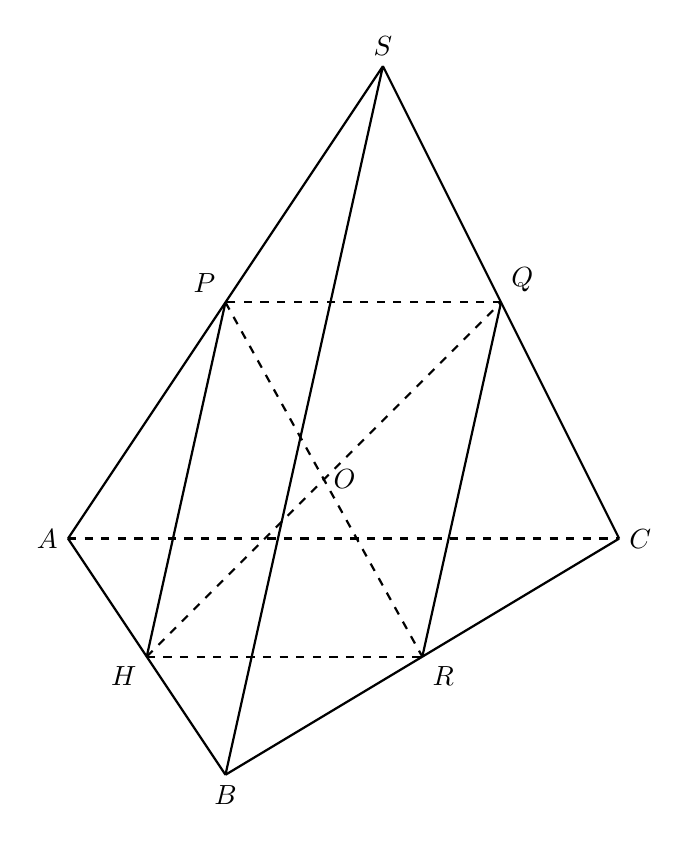
\begin{tikzpicture}
        \draw[-, thick] (2,0) node[anchor=north]{$B$} -- (7,3) node[anchor=west]{$C$}
                        (7,3)                         -- (4,9) node[anchor=south]{$S$}
                        (4,9)                         -- (0,3) node[anchor=east]{$A$}
                        (0,3)                         -- (2,0)
                        (2,0)                         -- (4,9);
        \draw[dashed, thick] (0,3) -- (7,3);
        \draw[dashed, thick] (5.5,6) node[anchor=south west]{$Q$} -- (2,6)     node[anchor=south east]{$P$}
                             (1,1.5) node[anchor=north east]{$H$} -- (4.5,1.5) node[anchor=north west]{$R$};
        \draw[-, thick] (4.5,1.5) -- (5.5,6)
                        (2,6) -- (1,1.5);
        \draw[dashed, thick] (2,6) -- (4.5,1.5)
                             (1,1.5) -- (5.5,6);
        \node[anchor=west] at (3.25,3.75) {$O$};
        %\draw[ultra thick, fill] (0,0) circle[radius=0.05];
      \end{tikzpicture}
      
      \caption{Середины четырёх рёбер тетраэдра.}
      \label{fig:tetrahedron}
    \end{figure}
  \end{solution}
  
  
  \begin{problem}[1.36]
    Имея радиус-векторы вершин треугольника $\bds r_1, \bds r_2, \bds r_3$, найти радиус-вектор центра окружности, вписанной в треугольник.
  \end{problem}
  
  \begin{solution}
    Пусть $O$~---~точка пересечения биссектрис $\triangle ABC$ (то есть центр вписанной окружности).
    Пусть $OH$~---~перпендикуляр, опущенный из $O$ к стороне $AC$ (то есть $|OH| \hm= r$, где $r$~---~радиус вписанной окружности) (\ref{fig:bisectors-intersection}).
    Обозначим угол $\angle BAC$ за $\alpha$: $\angle BAC \hm= \alpha$.
    
    \begin{figure}[h]
      \centering
      
      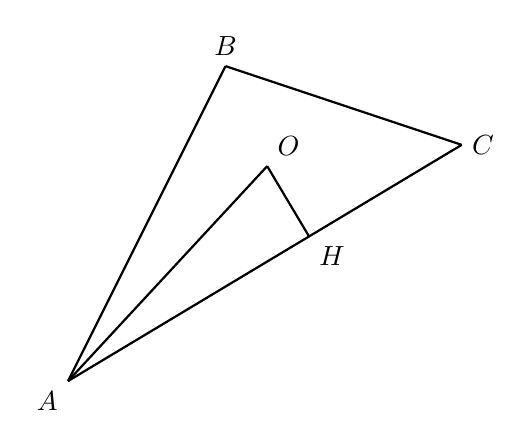
\begin{tikzpicture}
        \draw[-,thick] (0,0) node[anchor=north east]{$A$} -- (5,3) node[anchor=west]{$C$}
                       (5,3)                              -- (2,4) node[anchor=south]{$B$}
                       (2,4)                              -- (0,0);
        \draw[-,thick] (0,0)       -- (2.53,2.73) node[anchor=south west]{$O$}
                       (2.53,2.73) -- (3.06,1.84) node[anchor=north west]{$H$};
      \end{tikzpicture}
      
      \caption{Точка $O$ пересечения биссектрис $\triangle ABC$.}
      \label{fig:bisectors-intersection}
    \end{figure}
    
    Будем искать радиус вектор точки $O$ как $\vv O = \vv A + \vv{AO}$: положение $A$ известно, поэтому при таком пути решения надо получить $\vv{AO}$.

    \begin{figure}[h]
      \centering
      
      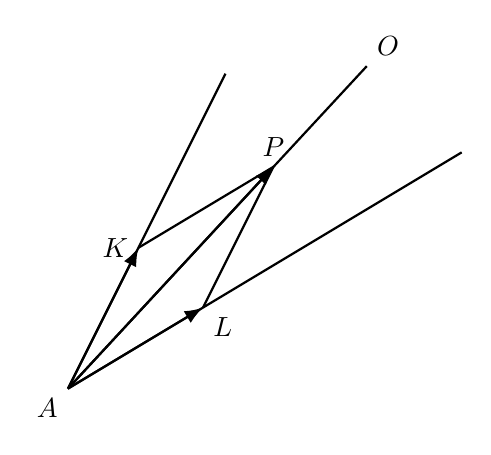
\begin{tikzpicture}
        \draw[-,thick] (0,0) node[anchor=north east]{$A$} -- (5,3)
                       (0,0)                              -- (2,4);
        \draw[-,thick]      (0,0)         -- (3.795,4.095) node[anchor=south west]{$O$};
        \draw[-Latex,thick] (0,0)         -- (1.714,1.028) node[anchor=north west]{$L$};  % (0.857,0.514)
        \draw[-,thick]      (1.714,1.028) -- (2.608,2.816) node[anchor=south]{$P$};       % (1.304,1.408)
        \draw[-Latex,thick] (0,0)         -- (0.894,1.788) node[anchor=east]{$K$};        % (0.447,0.894)
        \draw[-,thick]      (0.894,1.788) -- (2.608,2.816);
        \draw[-Latex,thick] (0,0)         -- (2.608,2.816);
      \end{tikzpicture}
      
      \caption{Вектор $\bds l \hm= \protect\vv{AP}$ в направлении прямой $AO$~---~сумма единичных векторов $\protect\vv{AK}$ и $\protect\vv{AL}$, направленных соответственно вдоль сторон $AB$ и $AC$ треугольника $ABC$.}
      \label{fig:l-parallel-ao}
    \end{figure}
    
    Начнём с того, что вектор в направлении прямой $AO$ (\ref{fig:l-parallel-ao}) можно получить как
    \begin{equation}\label{eq:l-vector}
      \bds l = \frac{\vv{AB}}{|AB|} + \frac{\vv{AC}}{|AC|}
    \end{equation}
    Но вектор не нормирован: $|\bds l| \hm{\not=} 1$.
    И сходу посчитать его модуль мы не можем (базис в задаче общий, не обязательно ортонормированный, поэтому скалярное произведение не выражается \emph{только} через компоненты векторов).
    Но модуль можно так выразить через угол $\alpha$ с помощью теоремы синусов для треугольника $APL$ (\ref{fig:l-parallel-ao}):
    \[
      \frac{AP}{\sin{\angle ALP}} = \frac{PL}{\sin{\angle PAL}}
    \]
    или, переходя к обозначениям $\bds l$ и $\alpha$ и пользуясь тем, что $|PL| \hm= 1$ по построению:
    \[
      \frac{|\bds l|}{\sin{(\pi - \alpha)}} = \frac{1}{\sin \frac{\alpha}{2}}
    \]
    В итоге получаем
    \begin{equation}\label{eq:l-module}
      |\bds l| = \frac{\sin \alpha}{\sin \frac{\alpha}{2}}
    \end{equation}
    
    Рассмотрим $\triangle AOH$ (\ref{fig:bisectors-intersection}).
    Сторона $AO$:
    \[
      AO = \frac{OH}{\sin \angle OAH} = \frac{r}{\sin \frac{\alpha}{2}}
    \]
    Вектор $\vv{AO}$:
    \[
      \vv{AO} = \frac{\bds l}{|\bds l|} \cdot |AO|
        \stackrel{(\ref{eq:l-module})}{=} \frac{\bds l}{\sin \alpha \Big/ \sin \frac{\alpha}{2}} \cdot \frac{r}{\sin \frac{\alpha}{2}}
        = \bds l \cdot \frac{r}{\sin \alpha}
        = \bigstar
    \]
    
    Радиус $r$ можно выразить через формулы для нахождения площади треугольника $\triangle ABC$:
    \[
      S_{\triangle ABC} = pr = \frac{1}{2} AC \cdot AB \cdot \sin \alpha
        \Rightarrow \frac{bc \sin \alpha}{2p}
    \]
    где $p$~---~полупериметр $\triangle ABC$, $b \hm\equiv AC$, $c \hm\equiv AB$.
    
    И тогда, возвращаясь к нахождению вектора $\vv{AO}$:
    \[
      \bigstar = \bds l \cdot \frac{r}{\sin \alpha}
        = \bds l \cdot \frac{bc}{2p}
        = \blacktriangledown
    \]
    
    Далее можно подставить вместо $\bds l$ его выражение через вектора $\vv{AC} \hm= \bds r_C \hm- \bds r_A$ и $\vv{AB} \hm= \bds r_B \hm- \bds r_A$ (\ref{eq:l-vector}) и вместо $p$ его выражение через длины сторон $\triangle ABC$ ($BC \hm\equiv a$):
    \[
      \blacktriangledown = \left(\frac{\bds r_C - \bds r_A}{b} + \frac{\bds r_B - \bds r_A}{c}\right) \cdot \frac{bc}{a + b + c}
        = \frac{c(\bds r_C - \bds r_A) + b(\bds r_B - \bds r_A)}{a + b + c}
    \]
    
    И в итоге для радиуса-вектора центра вписанной окружности $O$ получаем выражение:
    \[
      \bds r_O = \bds r_A + \vv{AO}
        = \frac{a \bds r_A + b \bds r_B + c \bds r_C}{a + b + c}
        = \frac{|\bds r_C - \bds r_B| \bds r_A + |\bds r_C - \bds r_A| \bds r_B + |\bds r_A - \bds r_B| \bds r_C}{|\bds r_C - \bds r_B| + |\bds r_C - \bds r_A| + |\bds r_A - \bds r_B|}
    \]
  \end{solution}
\end{document}
